\documentclass{article}
% \usepackage{../../lib/latex/draculatheme}
\usepackage{import}
\documentclass{article}
\usepackage[paper=letterpaper,margin=2cm]{geometry}
\usepackage[utf8]{inputenc}
\usepackage[russian]{babel}
\usepackage[]{graphicx}
\usepackage[usenames]{color}
\usepackage{colortbl}
\usepackage{geometry}
\usepackage{xcolor}
\usepackage{hyperref}
\usepackage{../../lib/latex/listings-rust}
\usepackage{fontspec}
\setmonofont{JetBrains Mono}[Contextuals=Alternate,Ligatures = TeX,]
\usepackage{listings}
\usepackage{keycommand}
\usepackage{caption}

\setmainfont[
  Ligatures=TeX,
  Extension=.otf,
  BoldFont=cmunbx,
  ItalicFont=cmunti,
  BoldItalicFont=cmunbi,
]{cmunrm}
\setsansfont[
  Ligatures=TeX,
  Extension=.otf,
  BoldFont=cmunsx,
  ItalicFont=cmunsi,
]{cmunss}

\geometry{
  a4paper,
  top=25mm,
  right=30mm,
  bottom=25mm,
  left=30mm
}

\hypersetup{
  colorlinks=true,
  linkcolor=blue!50!red,
  urlcolor=blue!70!black
}

\captionsetup[lstlisting]{
  font={tt},
}

% based on Atom One Light
\lstset{
  language=Java,
  frame=single,
  basicstyle=\ttfamily\color[HTML]{383a42},
  columns=fullflexible,
  breaklines=true,
  numbers=left,
  frame=tab,
  postbreak=\mbox{\textcolor{red}{$\hookrightarrow$}\space},
  extendedchars=false,
  showspaces=false,
  showstringspaces=false,
  identifierstyle=\ttfamily\color[HTML]{4078f2},
  commentstyle=\color[HTML]{a0a1a7},
  stringstyle=\color[HTML]{50a14f},
  keywordstyle=\color[HTML]{a626a4},
  numberstyle=\ttfamily\color[HTML]{2c91af},
  rulecolor=\color[HTML]{383a42}
}

\lstdefinelanguage{XML}
{
  morestring=[b]",
  morestring=[s]{>}{<},
  morecomment=[s]{<?}{?>},
}

\newcommand{\code}[1]{
  \lstset{title=#1}
  \lstinputlisting{#1}
}
\newkeycommand{\itmo}[variant=aboba, labn=aboba, discipline=aboba, group=aboba, student=aboba,teacher=aboba, year=2022]{
  \begin{titlepage}
    \begin{center}
      \section*{
        Федеральное государственное автономное образовательное учреждение\\ высшего образования\\
        «Национальный исследовательский университет ИТМО»\\
        Факультет Программной Инженерии и Компьютерной Техники \\
       }
      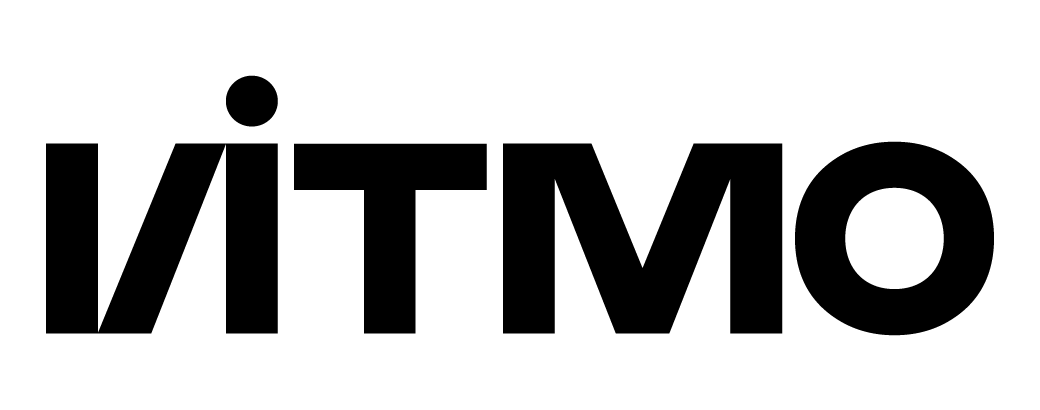
\includegraphics[scale=0.2]{../../lib/img/itmo.png}
    \end{center}

    \vspace{4cm}

    \begin{center}
      \large \textbf{Вариант \textnumero \commandkey{variant}}\\
      \textbf{Лабораторная работа \textnumero \commandkey{labn}}\\
      по дисциплине\\
      \textbf{\commandkey{discipline}}
    \end{center}

    \vspace*{\fill}

    \begin{flushright}
      Выполнил Студент группы \commandkey{group}\\
      \textbf{\commandkey{student}}\\
      Преподаватель: \\
      \textbf{\commandkey{teacher}}\\
    \end{flushright}

    \vspace{1cm}

    \begin{center}
      г. Санкт-Петербург\\
      \commandkey{year}г.
    \end{center}

    \thispagestyle{empty}
  \end{titlepage}
}



\begin{document}

\itmo[
  variant=1703,
  labn=8,
  discipline=Программирование,
  group=P3115,
  student=Владимир Мацюк,
  teacher=Кустарев Иван Павлович,
  year=2023,
  logo=../../lib/img/itmo.png
]

\section*{Задание}
\begin{itemize}
  \item Интерфейс должен быть реализован с помощью библиотеки JavaFX
  \item Графический интерфейс клиентской части должен поддерживать русский, финский, албанский и испанский (Мексика) языки / локали.
  \item Должно обеспечиваться корректное отображение чисел, даты и времени в соответстии с локалью.
  \item Переключение языков должно происходить без перезапуска приложения.
  \item Локализованные ресурсы должны храниться в файле свойств.
\end{itemize}
\section*{Доработать программу из лабораторной работы №7 следующим образом:}



Заменить консольный клиент на клиент с графическим интерфейсом пользователя(GUI). 
В функционал клиента должно входить:
\begin{enumerate}

  \item Окно с авторизацией/регистрацией.
  \item Отображение текущего пользователя.
  \item Таблица, отображающая все объекты из коллекции \begin{enumerate}
          \item Каждое поле объекта - отдельная колонка таблицы.
          \item Строки таблицы можно фильтровать/сортировать по значениям любой из колонок. Сортировку и фильтрацию значений столбцов реализовать с помощью Streams API.
        \end{enumerate}
  \item Поддержка всех команд из предыдущих лабораторных работ.
  \item Область, визуализирующую объекты коллекции \begin{enumerate}
          \item Объекты должны быть нарисованы с помощью графических примитивов с использованием Graphics, Canvas или аналогичных средств графической библиотеки.
          \item При визуализации использовать данные о координатах и размерах объекта.
          \item Объекты от разных пользователей должны быть нарисованы разными цветами.
          \item При нажатии на объект должна выводиться информация об этом объекте.
          \item При добавлении/удалении/изменении объекта, он должен автоматически появиться/исчезнуть/измениться  на области как владельца, так и всех других клиентов.
          \item При отрисовке объекта должна воспроизводиться согласованная с преподавателем анимация.
        \end{enumerate}
  \item Возможность редактирования отдельных полей любого из объектов (принадлежащего пользователю). Переход к редактированию объекта возможен из таблицы с общим списком объектов и из области с визуализацией объекта.
  \item Возможность удаления выбранного объекта (даже если команды remove ранее не было).
  \item Перед непосредственной разработкой приложения необходимо согласовать прототип интерфейса с преподавателем. Прототип интерфейса должен быть создан с помощью средства для построения прототипов интерфейсов(mockplus, draw.io, etc.)
\end{enumerate}

\section*{Исходный код}
\url{https://github.com/Wgmlgz/itmo2/tree/main/l8}

\section*{Вывод}
Во время выполнения работы я глубже ознакомился с ООП на языке java.
\end{document}
